\chapter{标题、摘要、引证、署名}\label{chap:other}
\section{标题}
文章的标题(如图~\ref{fig:title})简洁有力,以一句话文摘的形式反映了该文章研究的任务以及采用的方法这两项文章的精髓。标题的内容非常具体、准确、简练,均由术语构成,每个词都有明确的含义。在用词上,均采用名词短语,语法规范。

\begin{figure}[!htbp]
	\centering
	
\includegraphics[width=\textwidth]{title}
	\caption{文章的标题}
	\label{fig:title}
\end{figure}

\section{署名}
在署名的设计(如图~\ref{fig:signature})上,作者名称、单位以及邮箱采用不同的字体字号进行区分,并且排版工整,使得读者对于作者的信息一目了然。在署名的顺序上,可以看出,并不是按严格按名称首字母进行的排序,经过对作者的背景的研究,发现前两位作者是最后一位作者Hinton的学生,则署名顺序是以学生-导师的顺序完成,学生部分的署名按名称首字母的顺序排列。需要说明的是,由于该文章的三位作者都是深度学习领域公认的明星学者,因此该文章或许不存在所谓需要特别突出的“第一作者”。
\begin{figure}[!htbp]
	\centering
	
\includegraphics[width=\textwidth]{signature}
	\caption{文章的署名}
	\label{fig:signature}
\end{figure}

\section{摘要}
文章摘要的结构分析结果如图~\ref{fig:abstract}所示。

\begin{figure}[!htbp]
	\centering
	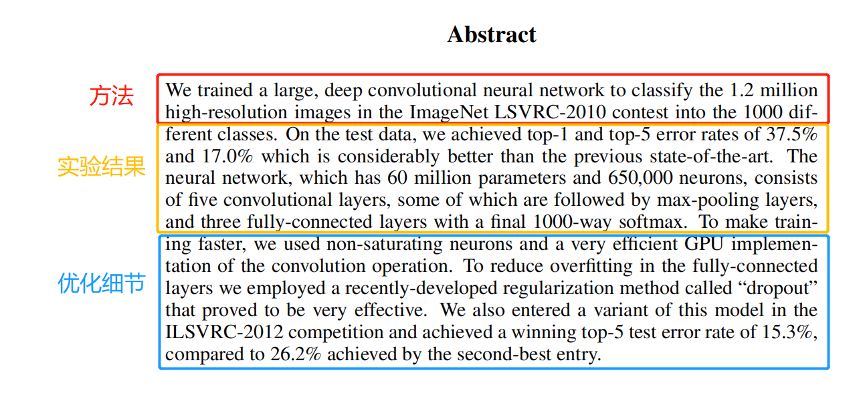
\includegraphics[width=\textwidth]{abstract}
	\caption{文章的摘要}
	\label{fig:abstract}
\end{figure}

在结构上,摘要采取了叙述文章采用的主要方法,即使用深度卷积神经网络进行图片分类,随后对实验结果进行了描述,最后通过叙述优化细节,来说明该文的方法是如何取得更优的效果。

这种摘要的结构是值得商榷的,一方面,对于大同行以及外行来说,这篇摘要并不完美,摘要并没有给出文章所面向的问题和研究意义,通过摘要无法对文章所面向的问题进行一个初步了解,如果将来论文需要面向大同行,建议将问题的背景进行补充;另一方面,对于小同行来说,这篇摘要已经能够充分反映研究中的必要信息,对于该文章所在领域来说,提高分类效率这一问题已经是此类与新模型相关的论文的共识性问题,关键在于新模型的结构以及效果如何,因此通过阅读这一摘要,即可清晰了解文章的工作及其意义。

在摘要内容的撰写方面,采用了简洁的纯文本进行叙述,语法上也没有较大的瑕疵,是值得肯定的。但摘要内容中出现了许多细节性数据,这一点是值得商榷的。摘要中给出了大量的细节性数据用于描述神经网络的模型架构、数据规模以及实验结果,显得不够简明扼要,如果将来论文需要面对大同行,建议将这些具体的实验数据略去,采用高度概括的词语进行叙述。但另一方面,对于小同行来说,根据这些细节性数据,已经可以较为全面的了解文章的工作以及效果。比如文章涉及领域面向大规模的图片分类问题,对于大同行来说,摘要中采用“大规模”这一概念描述即可,但对小同行来说,采用具体的数字规模说话,如该文中的“1.2 million”,更能直接反映文章模型的优势。此外,小同行还能够根据摘要中给出的一些模型关键参数的具体数值对文章设计的模型进行复现。

\section{引证}
对于引证部分,该文章均采用如图~\ref{fig:cited}所示的间接引用方式,引用的格式较为规范,参考文献的序号均紧跟在引证的主要内容后,且对于所引证的内容都通过简练的语言进行了转述,使之符合文章的表达情境。在文内的引用没有太大的问题,加之该文章作为深度学习领域的代表性论文,作者又是业界著名学者,其引证方式值得参考学习。
\begin{figure}[!htbp]
	\centering
	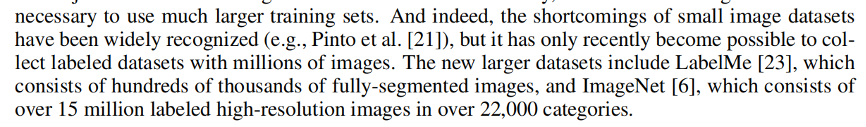
\includegraphics[width=\textwidth]{cited}
	\caption{文章中的引证示例}
	\label{fig:cited}
\end{figure}

对于引证的文献的范围来说,如图~\ref{fig:reference},可以看到,该文的引证范围较为全面,且参考文献的质量都较高。一方面,其覆盖了涉及领域早期的经典的奠基性文献,以及论文发表时期的最新研究成果;另一方面,其引用论文的质量较高,可以看到,引用文献许多来自于文章所属行业的顶级会议和顶级作者。此外,该文的引证文献均为公开文献,使得文章的引证是确实有据可查的。

\begin{figure}[!htbp]
	\centering
	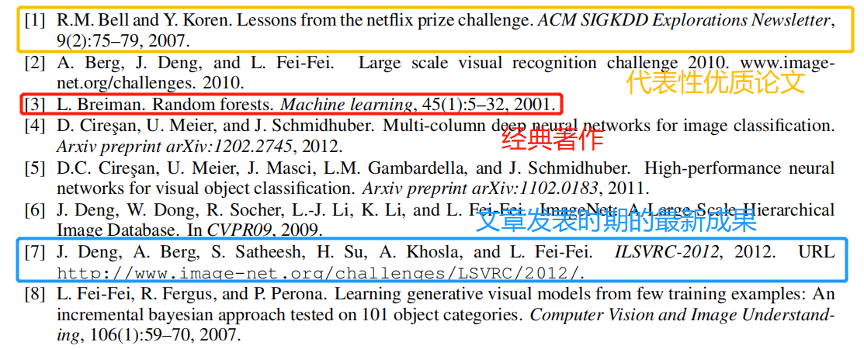
\includegraphics[width=\textwidth]{reference}
	\caption{文章的参考文献}
	\label{fig:reference}
\end{figure}
